\documentclass[a4paper, 12pt]{report}

\usepackage[utf8]{inputenc} 	% accents
\usepackage[T1]{fontenc}      	% caractères français
\usepackage{graphicx}		% images

\title{Projet INFO-H-303 : Villo!}
\author{Hereman Nicolas, Van Brande Rodrigue}
\date{24 avril 2015}

\begin{document}
\maketitle 

\section*{Diagramme entité-association} % Diagramme
	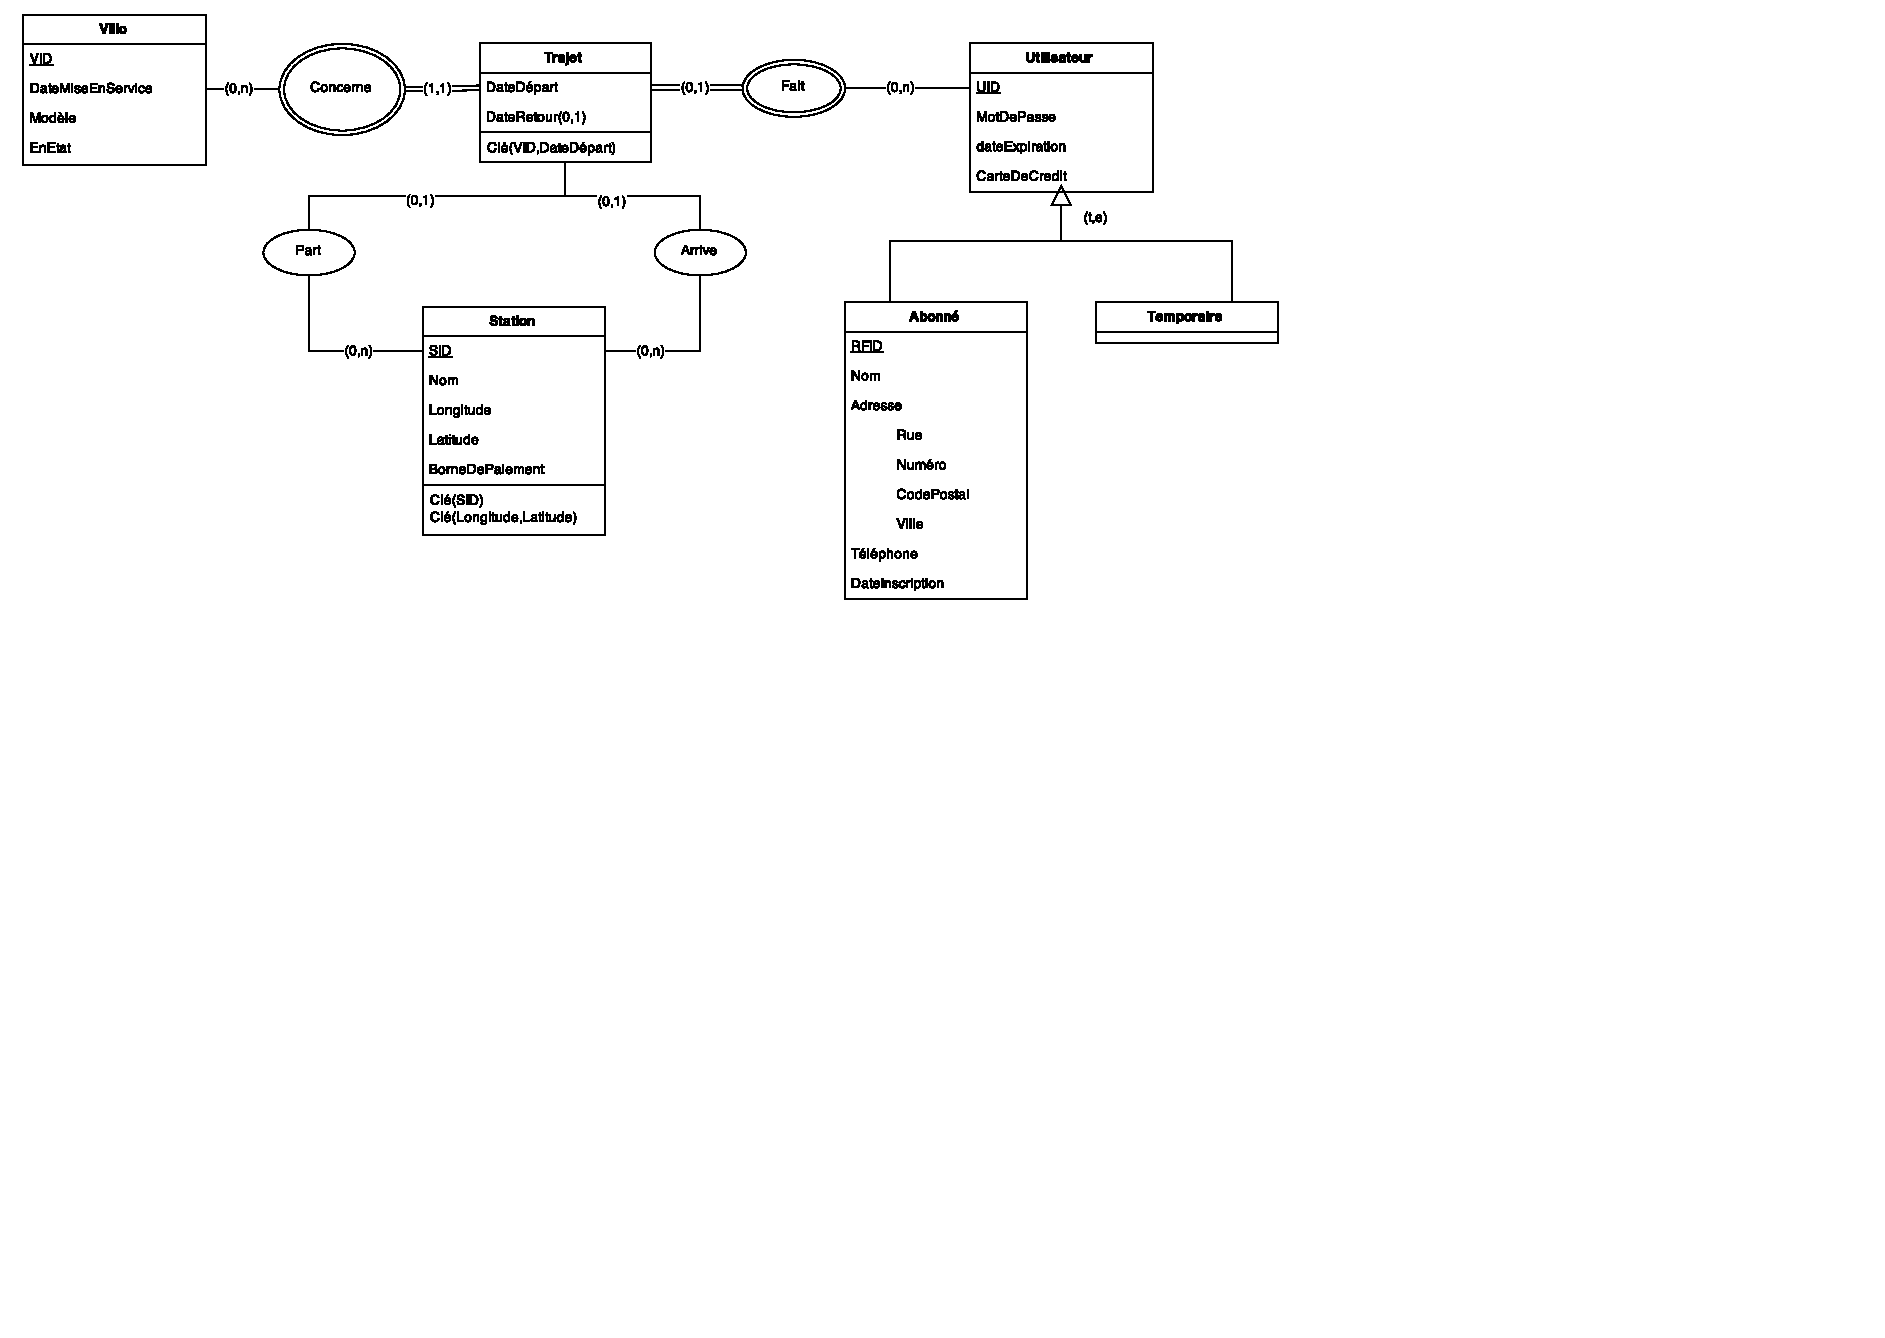
\includegraphics[scale=0.8]{entityassocdiagram.pdf}

\section*{Contraintes et hypothèses} %Contraintes

	\begin{itemize}
		\item La \textit{DateExpiration} d'un \textit{Abonné} doit être strictement supérieure à sa \textit{DateInscription}
		
		\item La \textit{DateDépart} d'un \textit{Trajet} doit être strictement supérieure à la \textit{DateInscription} de l'\textit{Abonné} qui le fait.
		
		\item La \textit{DateDépart} d'un \textit{Trajet} pot être strictement inférieure à la \textit{DateExpiration} de l'\textit{Utilisateur}.
		
		\item La \textit{DateDépart} d'un \textit{Trajet} doit être strictement inférieure à la \textit{DateExpiration} de l'\textit{Utilisateur} qui le fait.
		
		\item La \textit{DateRetour} d'un \textit{Trajet} doit être strictement supérieure à la \textit{DateDépart} de ce même \textit{Trajet}.
		
		\item La \textit{DateDépart} d'un \textit{Trajet} doit être strictement supérieure à la \textit{DateMiseEnService} du \textit{Villo} concerné.
		
		\item A l'instant \textit{DateRetour}, la \textit{Station} de retour d'un \textit{Trajet} doit contenir moins de \textit{Villos} que sa \textit{Capacité}. Le calcul du nombre de \textit{Villos} présents dans une \textit{Station} à l'aide de l'entité \textit{Trajet}.
		
		\item Un même \textit{Villo} ne peut pas concerner deux \textit{Trajets} en même temps.
		
		\item Un même \textit{Utilisateur} ne peut pas faire deux \textit{Trajets} en même temps.
		
		\item Un \textit{Trajet i} qui suit directement un autre \textit{Trajet j} pour un même \textit{Villo} doit avoir la même \textit{Station} de départ que la \textit{Station} d'arrivée du \textit{Trajet j}.
		
		% TODO: Rajouté des contraintes par rapport aux trajet avec des NULL
		
	\end{itemize}

\section*{Traduction relationnelle} %Relation
	
	\begin{itemize}
	
		\item Utilisateur(\underline{UID},MotDePasse,DateExpiration,CarteDeCredit)
		
		\item Abonne( \underline{UID}, \underline{RFID}, Nom, Rue, Numéro, CodePostal, Ville, Téléphone, DateInscription)
		
		\begin{itemize}
			\item UID référence Utilisateur.UID
		\end{itemize}
		
		\item Station(\underline{SID}, Nom, \underline{Longitude, Latitude}, Capacité, BorneDePaiement)
		
		\item Villo(\underline{VID},DateMiseEnService,Modèle, EnEtat)
		
		\item Trajet(\underline{VID,DateDépart}, \textit{UID}, \textit{StationDépart}, \textit{DateRetour}, \textit{StationRetour})
		
		\begin{itemize}
			\item UID référence Utilisateur.UID
			\item VID référence Villo.VID
			\item StationDépart référence Station.SID
			\item StationRetour référence Station.SID
		\end{itemize}
		
	\end{itemize}
	
	\subsection*{Remarque}
	Un Utilisateur.UID n'existant pas dans Abonné.UID est un utilisateur temporaire

\section*{Justification} % Justification

% TODO : MAJ les justifications
On a commencé par créer une table \textsc{utilisateur} pour stocker les données liées à ceux-ci.

Ensuite  on a hérité les abonnés des utilisateurs. On ajoute pas un héritage pour les utilisateurs temporaires, car toutes les données dont on a besoin pour ceux-ci sont déjà contenues dans la table \textsc{utilisateur}.

On a aussi besoin d'une table \textsc{station} afin d'enregistrer les données les concernant.

On a ensuite ajouté la table \textsc{velo}. Les vélos peuvent être liés à une station. Cela permet de savoir lequel est libre et lequel on peut donner à un utilisateur.

Pour terminer, on ajoute une table \textsc{deplacement} pour permettre de sauvegarder l'historique de tous les déplacements effectués. Celle ci est liée à la table \textsc{station} pour connaître l'endroit du départ et celui de l'arrivée. Elle est aussi liée à la table \textsc{velo} pour savoir quel vélo est utilisé et elle est aussi liée à la table \textsc{utilisateur} afin de savoir qui l'utilise.

\end{document}